\documentclass[12pt]{article}         
\usepackage{fullpage}
\usepackage[shortlabels]{enumitem}
\usepackage{amsmath}
\usepackage{graphicx}
\usepackage{amssymb}
\usepackage[utf8]{inputenc}
\usepackage{tikz}
\usepackage{caption}
\usetikzlibrary{automata, positioning, arrows}


\title{COMPSCI 250 Homework $\#$6}
\author{Aidan Chin \footnote{Adrian Nelson}}

\begin{document}
\maketitle

\section*{\textbf{P14.1.3} [10 pts]}
Suppose that $M_1$ and $M_2$ are two DFA’s with the same input alphabet. We’ll refer to the state set, start state, final state set, and transition function of $M_1$ as $S_1$, $\iota_1$, $F_1$, and $\delta_1$ respectively, and similarly for $M_2$. We define the \textbf{product DFA} $M_1 \times M_2$ as follows. The state set is the direct product $S_1 \times S_2$, the set of ordered pairs $\langle s_1, s_2 \rangle$ with $s_1 \in S_1$ and $s_2 \in S_2$. The start state is the pair $\langle \iota_1, \iota_2 \rangle$ and the final state set is $F_1 \times F_2$. The new transition function takes a state $\langle s_1, s_2 \rangle$ and a letter $a$ to $\langle \delta_1(s_1, a), \delta_2(s_2, a)\rangle$. Prove that the product DFA decides the language $L(M_1) \cap L(M_2)$.

\subsection*{\textbf{Solution:}}

solve using induction\newline
base case: the languages are both the empty set so start state is also the end state, and our product DFA is equivalent to each M1 and M2 because it too is also empty\newline
inductive hypothesis: for any string length n; $M1 \times M2$ decides the language $L(M1)\cap L(M2)$\newline
inductive step: suppose a non empty string w that is in the intersection of both languages, this means its accepted by M1 and M2; when processing w, M1 and M2 reach their respective final states which are in $F_1 \times F_2$, now suppose we have the same string but this time it ends in a letter $a$, which exists in $F_1\times F_2$ we do the same steps with w as before and get to s1, s2 which will be states just before the final state, and applying the transition function, we reach the DFA final state for both M1 and M2 and since w is accepted by both DFA it must be in the final states, proving that for each subsequent letter, there is a final state that can be reached if the string exists in both M1 and M2. this is spelling out the intersection of $L(M1)\cap L(M2)$

\newpage
\section*{\textbf{P14.2.5} [10 pts]}
A string in $\{a, \ldots , z\}^*$ is said to be a \textbf{palindrome} if it is equal to its own reversal. Examples of palindromes are \textit{madamimadam} and \textit{ablewasiereisawelba}. Is the set of palindromes decidable by a DFA? Prove your answer.


\subsection*{\textbf{Solution:}}

no there is not a DFA that can decide this, DFA is a finite state machine that must be able to be represented by a regular expression, but because these infinite length strings have no pattern for their first half (effectively random), which is effectively also infinite, but also need to match inversely in the second half, there is not a way to consider each of these patterns without a unique state for each one (they cannot be broken down into substrings), they cannot be represented using regular expressions, therefore cannot be represented using a DFA.
\newpage
\section*{\textbf{P14.5.8} [10 pts]}
The end of the section gives a recursive definition of the relation $\Delta^*(s, w, t)$ in a $\lambda$-NFA for arbitrary states $s$ and $t$, and arbitrary strings $w$. Prove by induction on this definition that if $\Delta^*(s, w, t)$ is true, then there exists a path in the $\lambda$-NFA’s state diagram from $s$ to $t$ such that the letter labels on the path, taken in order, spell out $w$.


\subsection*{\textbf{Solution:}}

we can prove this with induction\newline
base case: empty string, $\Delta(s, \emptyset, t)$ where there is a path from s to t that consumes no input\newline
hypothesis: for any string $w$ with length n, if $\Delta(s, w, t)$ is true then the path from s to t spells out w\newline
inductive step: if we use $w = xa$ where x is a string length n and a is just the letter a, if $\Delta(s, w, t)$ is true then there is a path from s to t that spells w. lets use y as an intermediate state in the path. by induction there must be a path from s to y that spells out x, also there must be one more edge that is a from y to t. therefore the entire path spells out xa, which is w

\newpage
\section*{\textbf{P14.6.4} [10 pts]}
In Problem 14.3.4\footnote{Let $k$ be a natural, let $\Sigma = \{a, b\}$, and consider the regular language $S_k = \Sigma^*a\Sigma^k$, consisting of all those strings whose $k + 1$’st to last letter exists and is an $a$. Find the minimal DFA for each such language $S_k$, and prove that it is minimal.} we defined the language $S = \Sigma^*a\Sigma^k$ of strings whose $k + 1$’st to last letter exists and is $a$. (Here $k$ is an arbitrary natural.) Design an NFA for this language with $k+2$ states and apply the Subset Construction to it. Minimize your DFA if necessary. You now have an example that will prove a theorem of the following form: For every $n$ with $n \geq n_0$, there exists a language that has an n-state ordinary NFA and whose minimal DFA has $f(n)$ states. You get to pick $n_0$, and the function $f(n)$ should be as large as you can make it.\footnote{Please check Piazza @996 for some additional notes on the problem.}


\subsection*{\textbf{Solution:}}

create the NFA M\newline
there will be k+2 states s0 s1 s2 ... sk+1\newline
s0 will loop on reading an a or b, and move onto s1 on reading an a\newline
sn will move to sn+1 on reading a letter in $\Sigma$ for 1 $\le$ n $\le$ k\newline
sk+1 is the final state with no outgoing transitions and only a pointing in\newline

converting the NFA M to a DFA M' using subset construction\newline
1. Initial State: lets denote the start state/ input state as s0\newline
2. Transitions: combining equivalent states, we find that most of the states do the same thing, loop on a or b and move on with a, so we only need 2 nodes to represent, moving to the end state on a, and looping on b, for the other node we loop on a and move back to start state on b\newline
3. Final State: any string that terminates on the final state (1) in the figure
\begin{figure}[h]
    \centering
    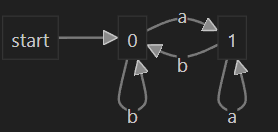
\includegraphics[width=.5\linewidth]{Screenshot 2024-05-10 201301.png}
\end{figure}

\newpage
\section*{\textbf{P14.7.5} [10 pts]}
Here is another way to modify a $\lambda$-NFA. For every letter move $\langle s, x, t \rangle$, where $x$ is a letter in $\Sigma$, add a corresponding $\lambda$-move $\langle s, \lambda, t \rangle$. Keep the start state and final state set the same.

\begin{enumerate}[(a)]
    \item Describe a three-state ordinary NFA whose language is $\{ab\}$. Apply this modification to your NFA and describe the result. What is the language of the modified $\lambda$-NFA?

    \item If this modification is applied to a $\lambda$-NFA with language $L$, what is the resulting language?

\end{enumerate}


\subsection*{\textbf{Solution:}}
\begin{enumerate}[(a)]
    \item to find out the language we need to consider all possible paths, but because the lambda steps skip the letter, the language is now a+b+ab
    \begin{figure}[h]
        \centering
        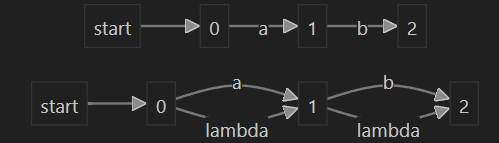
\includegraphics[width=.5\linewidth]{fig2.png}
    \end{figure}

    \item if this modification is applied to a $\lambda$-NFA with language $L$, each transition state can be skipped therefore the empty set, each individual letter, and all combinations of letters in the same order, with just deletions will be in L, for example if L = abc in that order, then there will be a, b, c, ab, ac, bc, abc in the new set
\end{enumerate}


\newpage
\section*{\textbf{P14.8.9} [10 pts]}
Formally prove the correctness of our construction for the star operator, as follows. Let $N$ be a $\lambda$-NFA constructed for the regular expression $\alpha$, and let $N'$ be the one constructed for $\alpha^*$, with two new states and four new $\lambda$-moves. Let $L$ be the language of $\alpha$.

\begin{enumerate}[(a)]
    \item By induction on all naturals $t$, prove that if $w$ is any string in the language $L^t$, then there are $w$-paths from the start state of $N'$ to both the original final state of $N$ and to the final state of $N'$. (The path to $N$’s final state is a useful inductive hypothesis.)

    \item Prove, by induction on all paths from the start state of $N'$ to either the original start state of $N$, the original final state of $N$, or the final state of $N'$, that the string read on the path is in the language $L^*$.

\end{enumerate}

\subsection*{\textbf{Solution:}}
\begin{enumerate}[(a)]
    \item base case: t = 0, where L will be the empty set, w will be length 0 and N $\&$ N' will be also length 0\newline
    inductive hypothesis: if $w$ is any string in the language $L^t$, then there are $w$-paths from the start state of $N'$ to both the original final state of $N$ and to the final state of $N'$. \newline
    inductive step: let w be any string in L k+1 which can be expressed as xy where x is a string in Lk and y is a string in L, using the hypothesis we already know that there exists x paths from start of N' to both original final state in N and final state of N', also since Y is in L there exists a path y from the start state of N' to the final state of N'. concatenating these paths we can create w paths from the start state of N' to both the original final state N and the final of N'

    \item same base case, meaning that the empty string exists in L, also we utilize the previous inductive step, which already state for an k, if w is in Lk there is w paths from the start state of N' to both the original final state of N and the final state of N'
\end{enumerate}


\newpage
\section*{\textbf{P14.10.2} [10 pts]}
Build successively a $\lambda$-NFA, an NFA, a DFA, and a minimal DFA from the regular expression in Exercise 14.10.3\footnote{Design a DFA whose language is the set of strings in $\{a, b\}^*$ that have a number of $a$’s divisible by 3. Use the state elimination construction to obtain a regular expression for this language.}. Before making the ordinary NFA, simplify the $\lambda$-NFA to an equivalent one with six states, using loops for the $a^*$ components. \\
Note: We will give you the $\lambda$-NFA to start with. \\
\begin{center}
    \begin{tikzpicture}[shorten >=1pt,node distance=3cm,on grid,auto] 
       \node[state,initial] (1)  {$1$};
       \node[state] (2) [right=of 1]  {$2$}; 
       \node[state] (3) [below=of 2] {$3$}; 
       \node[state] (4) [right=of 3] {$4$}; 
       \node[state] (5) [right=of 2] {$5$};
       \node[state,accepting] (6) [right=of 5] {$6$};
        \path[->] 
        (1) edge  node {$\lambda$} (2)
        (2) edge  node [swap] {$a$} (3)
            edge node [swap] {$b$} (5)
            edge [bend right] node [swap] {$\lambda$} (5)
        (3) edge  node  {$a$} (4)
            edge [loop below]  node  {$b$} (3)
        (4) edge  node [swap] {$a$} (5) 
            edge [loop below]  node  {$b$} (4) 
        (5) edge  node {$\lambda$} (6)
            edge [bend right] node [swap] {$\lambda$} (2);
    \end{tikzpicture}
    \captionof{figure}{$\lambda$-NFA for $(b + ab^*ab^*a)^*)$} \label{1}
\end{center}


\subsection*{\textbf{Solution:}}
\begin{center}
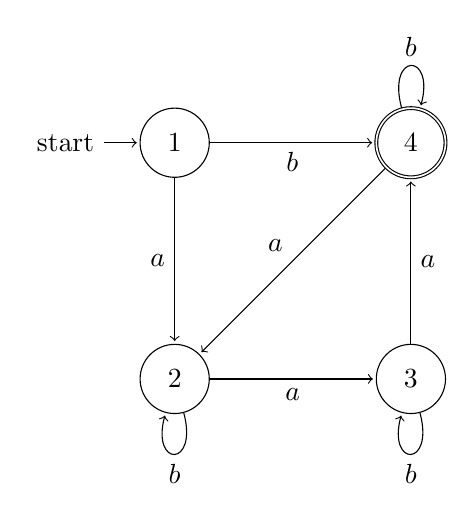
\begin{tikzpicture}[shorten >=1pt,node distance=3cm,on grid,auto] 
    \node[state,initial] (1) {$1$}; 
    \node[state] (2) [below=of 1] {$2$}; 
    \node[state] (3) [right=of 2] {$3$}; 
    \node[state,accepting] (4) [right=of 1] {$4$};
    \path[->] 
        (1) edge node [swap] {$a$} (2)
            edge node [swap] {$b$} (4)
        (2) edge node [swap] {$a$} (3)
            edge [loop below] node {$b$} (2)
        (3) edge node [swap] {$a$} (4)
            edge [loop below] node {$b$} (3)
        (4) edge node [swap] {$a$} (2)
            edge [loop above] node {$b$} (4);
    \end{tikzpicture}
    \end{center}
    \captionof{figure}{NFA $\&$ DFA for $(b + ab^*ab^*a)^*)$} \label{2}
states 2 and 3 are equivalent so combine them, 1 and 4 are also equivalent so combine them
\begin{center}
    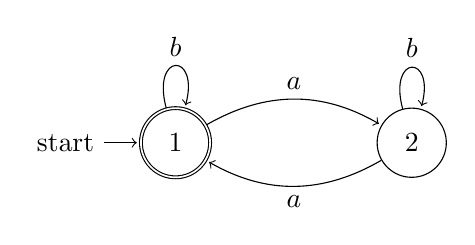
\begin{tikzpicture}[shorten >=1pt,node distance=3cm,on grid,auto] 
        \node[state, initial, accepting] (1) {$1$}; 
        \node[state] (2) [right=of 1] {$2$};
        \path[->] 
            (1) edge [bend left] node {$a$} (2)
                edge [loop above] node {$b$} (1)
            (2) edge [bend left] node {$a$} (1)
                edge [loop above] node {$b$} (2);


    \end{tikzpicture}
    \end{center}
    \captionof{figure}{Minimized DFA for $(b + ab^*ab^*a)^*)$} \label{3}

\newpage
\section*{\textbf{EC: P14.10.10 (a, b)} [10 pts]}
In Problem 5.5.1\footnote{If $L$ is a language and $a$ is a letter, we define the \textbf{quotient of} $L$ \textbf{by} $a$, written $La^{-1}$, as follows. $La^{-1}$ consists of all those strings that $would$ $be$ in $L$ $if$ you appended an $a$ to them --- formally, $La^{-1}$ = $\{w : wa \in L\}$. Prove that if $S$ is any regular expression, and $a$ is any letter, then $L(S)a^{-1}$ is a regular language. Give a recursive algorithm to produce a regular expression for this language.} we defined the \textbf{quotient} of a language $L$ by a letter $a$, so that the language $La^{-1}$ was defined to be the set $\{w : wa \in L\}$. We proved there that we could take a regular expression $\alpha$ and produce a regular expression for $L(\alpha)a^{-1}$.

\begin{enumerate}[(a)]
    \item The quotient of a language $L$ by a string $w$ is the set $Lw^{-1} = \{u : uw \in L\}$. Argue using the result of Problem 5.5.1 that $Lw^{-1}$ must be regular if $L$ is regular and $w$ is any string.

    \item Let $D$ be a DFA for a language $L$ and let $w$ be any string over $D$’s alphabet. Argue that there is a DFA $D'$, whose language is $Lw^{-1}$, that can be obtained from $D$ by simply changing the final state set.
\end{enumerate}

\subsection*{\textbf{Solution:}}


\newpage
\section*{\textbf{EC: P15.6.1} [10 pts]}
Build a Turing machine $M_{shift}$ that when started on input $w$ (i.e., in configuration $\iota \square w$), halts with tape contents $\square \square wh \square$. Let $\Sigma = \{a, b\}$.

\subsection*{\textbf{Solution:}}



\end{document} 